\documentclass[10pt,pdf,hyperref={unicode}]{beamer}
\mode<presentation>
\usetheme{AnnArbor}
\usecolortheme{beaver}
\usepackage[utf8]{inputenc}
\usepackage[english,russian]{babel}
\usepackage{amssymb}
\usepackage{graphicx}
\usepackage{epstopdf}
\usepackage[english]{isodate}
\usepackage[noend]{algorithmic}
\usepackage{algorithm}
\usepackage[T2A]{fontenc}

\title[Strategy-profness versus...]{Strategy-proofness versus Efficiency in Matching with Indifferences: Redesigning the NYC High School Match}
\author[БЕЗЕР]{Бажанов К.Н., Егурнов А.А., Зрянина М.С., Егурнов Д.А., Рыжакова Е.В.}
\institute[НИУ ВШЭ]{Национальный Исследовательский Университет Высшая Школа Экономики}
\date{14 Марта 2013}

\begin{document}

\begin{frame}
    \titlepage
\end{frame}

\begin{frame}
    \frametitle{Содержание}
    \tableofcontents
\end{frame}

\AtBeginSection[]
{
    \begin{frame}
        \frametitle{Содержание}
        \tableofcontents[currentsection]
    \end{frame}
}

\AtBeginSubsection[]
{
    \begin{frame}
        \frametitle{Содержание}
        \tableofcontents[currentsection, currentsubsection]
    \end{frame}
}

\section{Об авторах}

\begin{frame}
    \frametitle{Atila Abdulkadiroglu}
    \begin{columns}
        \begin{column}{.5\textwidth}
            \scriptsize{
            \begin{itemize}
                \item Department of Economics at Duke University 2006 -- $\dots$
                \item Northwestern University and Columbia University $\dots$ -- 2006
                \item PhD in Economics at the University of Rochester
                \item Recipient of an Alfred P. Sloan Research Fellowship
                \item Recipient of and National Science Foundation CAREER award
                \item Editor-in-Chief of Review of Economic Design
                \item Serves on the board of The Institute for Innovation in Public School Choice
                \item He has consulted several school districts in redesigning student assignment systems, including Boston (MA), Chicago (Il), Denver (CO), New Orleans (LA), New York City (NY)
                \item His research has led to the design and implementation of better admissions policies in school choice programs in the US
                \item His current research also focuses on economics of education.
            \end{itemize}
            }
        \end{column}
        \begin{column}{.5\textwidth}
            \begin{figure}[H]
                \noindent\centering{
                    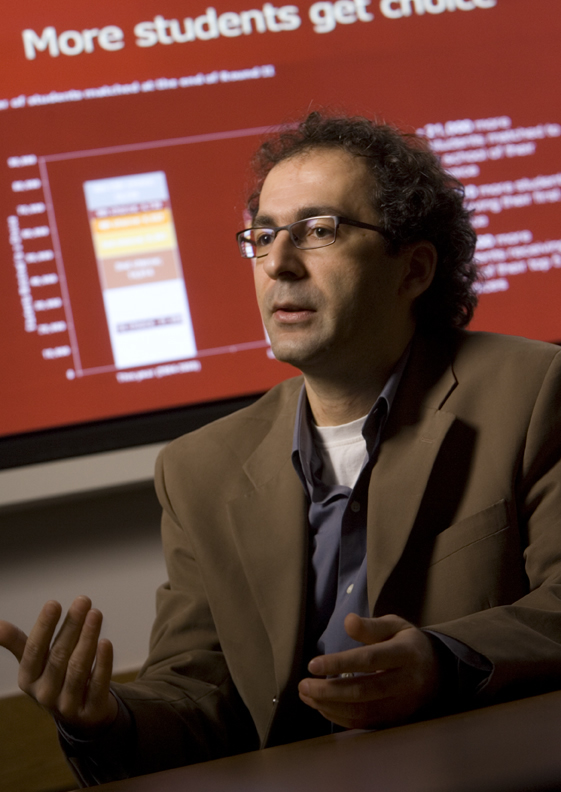
\includegraphics[height = 55mm]{figures/atilaa.jpeg}
                }
            \end{figure}
        \end{column}
    \end{columns}
\end{frame}

\begin{frame}
    \frametitle{Parag Pathak}
    \begin{columns}
        \begin{column}{.5\textwidth}
            \begin{itemize}
                \item A.B., Harvard, summa cum laude in Applied Mathematics, 2002
                \item Ph.D., Harvard, Business Economics, 2003-2007.
                \item National Bureau of Economic Research, 2008 - $\dots$
                \item Massachusetts Institute of Technology, 2008 - $\dots$
                \item NSF Presidential Early Career Award for Scientists and Engineers, 2012.
                \item Alfred P. Sloan Research Fellow, 2012-2013
            \end{itemize}
        \end{column}
        \begin{column}{.5\textwidth}
            \begin{figure}[H]
                \noindent\centering{
                    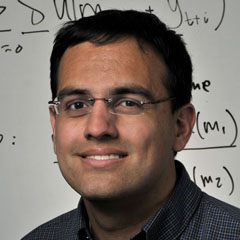
\includegraphics[height = 55mm]{figures/parag.jpeg}
                }
            \end{figure}
        \end{column}
    \end{columns}
\end{frame}

\begin{frame}
    \frametitle{Alvin E. Roth}
    \begin{columns}
        \begin{column}{.5\textwidth}
            \scriptsize{
            \begin{itemize}
                \item Received his Ph.D at Stanford University
                \item Was the Andrew Mellon Professor of Economics.
                \item Has been a Guggenheim and Sloan fellow.
                \item He is a Fellow of the American Academy of Arts and Sciences and the Econometric Society
                \item Chair of the American Economic Association's Ad Hoc Committee on the Job Market
                \item George Gund Professor of Economics and Business Administration in the Department of Economics at Harvard University, and in the Harvard Business School.
                \item His interests are in game theory, experimental economics, and market design.
                \item He has recently been involved in the reorganization of the market for Gastroenterology fellows.
                \item He is one of the founders and designers of the New England Program for Kidney Exchange, for incompatible patient-donor pairs.
            \end{itemize}
            }
        \end{column}
        \begin{column}{.5\textwidth}
            \begin{figure}[H]
                \noindent\centering{
                    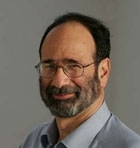
\includegraphics[height = 55mm]{figures/alvin.jpeg}
                }
            \end{figure}
        \end{column}
    \end{columns}
\end{frame}

\section{Постановка задачи}

\begin{frame}
    \frametitle{Причина возникновения задачи}
    \begin{block}{Причины}
        \begin{itemize}
            \item Огромное количество школ и абитуриентов\\В 2003-2004 более 90000 абитуриентов.
            \item Старый {\bf децентрализованный} механизм
            \item Школы имели склонность занижать {\bf квоты}
        \end{itemize}
    \end{block}
\end{frame}

\begin{frame}
    \frametitle{Особенности старой модели}
    \begin{block}{Ограничения на предпочтения}
        \begin{itemize}
            \item Школьники могут выбрать только 12 школ
            \item Многие школы ранжируют школьников {\bf пассивно}
        \end{itemize}
    \end{block}

    \begin{block}{Всего три тура}
        \begin{itemize}
            \item В первом туре участвуют только спецшкольники
            \item Оставшиеся места разыгрываются во втором (основном) туре
            \item Нераспределенные школьники могут выбрать ещё 12 школ
        \end{itemize}
    \end{block}

    \begin{block}{Требования в к новому механизму}
        \begin{itemize}
            \item Устойчивасть
            \item Эффективность
            \item Неманипулируемость
        \end{itemize}
    \end{block}
\end{frame}

\begin{frame}
    \frametitle{Модель}
    \begin{itemize}
        \item $I$ -- {\bf множество учеников}
        \item $S$ -- {\bf множество школ}
        \item $q_S$ -- количество мест в школе ({\bf квота})
        \item $P_i$ -- отношение строгого порядка на множестве $S \cup \left\{i\right\}$ (задаёт {\bf предпочтения ученика} $i$)
        \item Школа $s$ {\bf допустима} для ученика $i$, если $s P_i i$.
        \item $R_i$ -- отношение слабого порядка на множестве $I \cup \left\{s\right\}$ (задаёт {\bf предпочтения} $s$)
        \item Ученик $i$ {\bf допустим} для школы $s$, если $i R_s s$.
    \end{itemize}
\end{frame}

\begin{frame}
    \frametitle{Модель}
    \begin{itemize}
        \item Паросочетание $\mu$ {\bf индивидуально рационально} если каждому агенту сопоставляется допустимый агент
        \item Пара $(i, s)$ {\bf блокирующая} если $s P_i \mu(i)$ и либо $|\mu(s)| < q_s$ и $i R_s s$, либо  $\exists i^\prime \in I: i R_s i^\prime$
        \item Паросочетание {\bf доминирует} $\nu$ если $\forall i \in I: \mu(i) R_i \nu(i)$ и $\exists i \in I: \mu(i) P_i \nu(i)$
        \item $\mu$ {\bf стабильно} если оно {\bf индивидуально рационально} и не имеет {\bf блокирующих пар}
        \item $\mu$ {\bf оптимально для абитуриента} если оно не доминируется никаким другим стабильным паросочетанием
        \item $\mu$ {\bf эффективно} если оно не доминируется никаким другим паросочетанием
    \end{itemize}
\end{frame}

\begin{frame}
    \frametitle{Модель}
    \begin{block}{Определение}
        $\phi: (P_I, R_S) \longmapsto \mu$ -- {\bf прямой механизм} 
    \end{block}

    \begin{block}{Определение}
        Механизм $\phi$ {\bf dominant strategy incentive compatible (DSIC)} для школьника $i$ если $\forall (R_I, R_S), \forall P_i^\prime: \phi_i(P_I; R_S) R_i \phi(P_i^\prime, P_{-i}; R_S)$
    \end{block}

    \begin{block}{Определение}
        Механизм называется {\bf неманипулируемым (strategy proof)} если DSIC выполняется для всех абитуриентов.
    \end{block}
\end{frame}

\section{Алгоритм Deferred Acceptance}

\begin{frame}
    \frametitle{Алгоритм Deferred Acceptance (DA)}
    \begin{block}{Описание алгоритма}
        {\bf Шаг 1:} Каждый ученик выбирает школу, которая нравится ему больше всего. Каждая школа бронирует место за учениками, которые выбрали её в порядке, который соответствует её предпочтениям. Если желающих оказалось больше, чем позволяет квота, то школа отказывает им и эти ученики остаются не приписанными ни к одной школе.\\
        $\dots$\\
        {\bf Шаг k:} Каждый ученик, которому было отказано на предыдущем шаге, выбирает следующую школу из своего списка предпочтений. После того, как все ученики сделали свой выбор, школа рассматривает множество учеников, которым забронировано место, и тех, кто только подал заявку, и оставляет в соответствии со своими предпочтениями только тех, кто попадает в её квоту.\\
        $\dots$\\
        Алгоритм завершается тогда, когда у каждого ученика есть школа, которая забронировала для него место. К этой школе он и будет приписан в итоге.
    \end{block}
\end{frame}

\begin{frame}
    \frametitle{Разрешение неопределенностей (tiebreaking)}
    \begin{block}{ }
        \begin{itemize}
        \item STB -- single tie breaking -- каждому студенту приписывается номер, использующийся для разрешения неопределенности во всех школах.
        \item MTB -- mutiple tie breaking -- в каждой школе используется своя нумерация.
        \end{itemize}
    \end{block}

    \begin{figure}[H]
        \noindent\centering{
            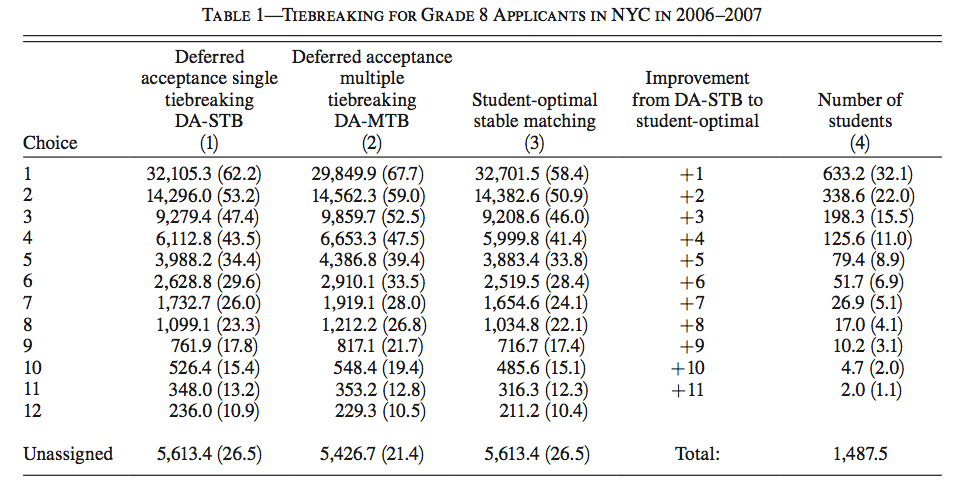
\includegraphics[height = 55mm]{figures/table-tiebreaking.png}
        }
    \end{figure}
\end{frame}

\begin{frame}
    \frametitle{Утверждения}
    \begin{block}{Утверждение 1}
        Если паросочетание $\mu$ является оптимальным для абитуриента, тогда не существует индивидуально-рациональное паросочетание $\nu$ (может быть и не стабильным) такое, что $\forall i \in I: \nu(i) P_i \mu(i)$.
    \end{block}

    \begin{block}{Утверждение 2}
        Для любого профиля предпочтений $(P_I, R_S)$ любое паросочетание, которое может быть получено с помощью MTB, но не STB не является оптимальным для абитуриента стабильным паросочетанием.
    \end{block}

    \begin{block}{Теорема}
        Не существует механизма, который был бы неманипулируемым и доминировал бы DA с STB или MTB.
    \end{block}
\end{frame}

\begin{frame}
    \frametitle{Замечания}
    \begin{block}{Замечание 1}
        Разрешение безразличий не всегда приводит к оптимальному для студентов стабильному паросочетанию.
    \end{block}

    \begin{block}{Замечание 2}
        Выигрыш в полезности возможен только за счет потери неманипулируемости.
    \end{block}
\end{frame}

\section{Заключение}

\begin{frame}
    \frametitle{Заключение}
    \begin{block}{ }
        \begin{itemize}
            \item Популярные программы увеличи свои квоты
            \item Популярные направления стали ранжировать более число студентов
            \item Strategy-proofness = данные для социологичесикх исследований
            \item Непопулярные школы были закрыты
        \end{itemize}
    \end{block}
\end{frame}

\begin{frame}
    \begin{center}
        {\Large Спасбо за внимание!}
    \end{center}

    \begin{center}
        {\Large Вопросы?}
    \end{center}
\end{frame}

\end{document}
